% Options for packages loaded elsewhere
\PassOptionsToPackage{unicode}{hyperref}
\PassOptionsToPackage{hyphens}{url}
\PassOptionsToPackage{dvipsnames,svgnames,x11names}{xcolor}
%
\documentclass[
  letterpaper,
  DIV=11,
  numbers=noendperiod]{scrartcl}

\usepackage{amsmath,amssymb}
\usepackage{iftex}
\ifPDFTeX
  \usepackage[T1]{fontenc}
  \usepackage[utf8]{inputenc}
  \usepackage{textcomp} % provide euro and other symbols
\else % if luatex or xetex
  \usepackage{unicode-math}
  \defaultfontfeatures{Scale=MatchLowercase}
  \defaultfontfeatures[\rmfamily]{Ligatures=TeX,Scale=1}
\fi
\usepackage{lmodern}
\ifPDFTeX\else  
    % xetex/luatex font selection
\fi
% Use upquote if available, for straight quotes in verbatim environments
\IfFileExists{upquote.sty}{\usepackage{upquote}}{}
\IfFileExists{microtype.sty}{% use microtype if available
  \usepackage[]{microtype}
  \UseMicrotypeSet[protrusion]{basicmath} % disable protrusion for tt fonts
}{}
\makeatletter
\@ifundefined{KOMAClassName}{% if non-KOMA class
  \IfFileExists{parskip.sty}{%
    \usepackage{parskip}
  }{% else
    \setlength{\parindent}{0pt}
    \setlength{\parskip}{6pt plus 2pt minus 1pt}}
}{% if KOMA class
  \KOMAoptions{parskip=half}}
\makeatother
\usepackage{xcolor}
\setlength{\emergencystretch}{3em} % prevent overfull lines
\setcounter{secnumdepth}{-\maxdimen} % remove section numbering
% Make \paragraph and \subparagraph free-standing
\makeatletter
\ifx\paragraph\undefined\else
  \let\oldparagraph\paragraph
  \renewcommand{\paragraph}{
    \@ifstar
      \xxxParagraphStar
      \xxxParagraphNoStar
  }
  \newcommand{\xxxParagraphStar}[1]{\oldparagraph*{#1}\mbox{}}
  \newcommand{\xxxParagraphNoStar}[1]{\oldparagraph{#1}\mbox{}}
\fi
\ifx\subparagraph\undefined\else
  \let\oldsubparagraph\subparagraph
  \renewcommand{\subparagraph}{
    \@ifstar
      \xxxSubParagraphStar
      \xxxSubParagraphNoStar
  }
  \newcommand{\xxxSubParagraphStar}[1]{\oldsubparagraph*{#1}\mbox{}}
  \newcommand{\xxxSubParagraphNoStar}[1]{\oldsubparagraph{#1}\mbox{}}
\fi
\makeatother


\providecommand{\tightlist}{%
  \setlength{\itemsep}{0pt}\setlength{\parskip}{0pt}}\usepackage{longtable,booktabs,array}
\usepackage{calc} % for calculating minipage widths
% Correct order of tables after \paragraph or \subparagraph
\usepackage{etoolbox}
\makeatletter
\patchcmd\longtable{\par}{\if@noskipsec\mbox{}\fi\par}{}{}
\makeatother
% Allow footnotes in longtable head/foot
\IfFileExists{footnotehyper.sty}{\usepackage{footnotehyper}}{\usepackage{footnote}}
\makesavenoteenv{longtable}
\usepackage{graphicx}
\makeatletter
\def\maxwidth{\ifdim\Gin@nat@width>\linewidth\linewidth\else\Gin@nat@width\fi}
\def\maxheight{\ifdim\Gin@nat@height>\textheight\textheight\else\Gin@nat@height\fi}
\makeatother
% Scale images if necessary, so that they will not overflow the page
% margins by default, and it is still possible to overwrite the defaults
% using explicit options in \includegraphics[width, height, ...]{}
\setkeys{Gin}{width=\maxwidth,height=\maxheight,keepaspectratio}
% Set default figure placement to htbp
\makeatletter
\def\fps@figure{htbp}
\makeatother

\usepackage{float}
\usepackage{tabularray}
\usepackage[normalem]{ulem}
\usepackage{graphicx}
\UseTblrLibrary{booktabs}
\UseTblrLibrary{rotating}
\UseTblrLibrary{siunitx}
\NewTableCommand{\tinytableDefineColor}[3]{\definecolor{#1}{#2}{#3}}
\newcommand{\tinytableTabularrayUnderline}[1]{\underline{#1}}
\newcommand{\tinytableTabularrayStrikeout}[1]{\sout{#1}}
\KOMAoption{captions}{tableheading,figureheading}
\makeatletter
\@ifpackageloaded{caption}{}{\usepackage{caption}}
\AtBeginDocument{%
\ifdefined\contentsname
  \renewcommand*\contentsname{Table of contents}
\else
  \newcommand\contentsname{Table of contents}
\fi
\ifdefined\listfigurename
  \renewcommand*\listfigurename{List of Figures}
\else
  \newcommand\listfigurename{List of Figures}
\fi
\ifdefined\listtablename
  \renewcommand*\listtablename{List of Tables}
\else
  \newcommand\listtablename{List of Tables}
\fi
\ifdefined\figurename
  \renewcommand*\figurename{Figure}
\else
  \newcommand\figurename{Figure}
\fi
\ifdefined\tablename
  \renewcommand*\tablename{Table}
\else
  \newcommand\tablename{Table}
\fi
}
\@ifpackageloaded{float}{}{\usepackage{float}}
\floatstyle{ruled}
\@ifundefined{c@chapter}{\newfloat{codelisting}{h}{lop}}{\newfloat{codelisting}{h}{lop}[chapter]}
\floatname{codelisting}{Listing}
\newcommand*\listoflistings{\listof{codelisting}{List of Listings}}
\makeatother
\makeatletter
\makeatother
\makeatletter
\@ifpackageloaded{caption}{}{\usepackage{caption}}
\@ifpackageloaded{subcaption}{}{\usepackage{subcaption}}
\makeatother

\ifLuaTeX
  \usepackage{selnolig}  % disable illegal ligatures
\fi
\usepackage{bookmark}

\IfFileExists{xurl.sty}{\usepackage{xurl}}{} % add URL line breaks if available
\urlstyle{same} % disable monospaced font for URLs
\hypersetup{
  pdftitle={When Science Strikes Back},
  pdfauthor={Gabriel Caser dos Passos and Nelson Ricardo Laverde Cubillos},
  colorlinks=true,
  linkcolor={blue},
  filecolor={Maroon},
  citecolor={Blue},
  urlcolor={Blue},
  pdfcreator={LaTeX via pandoc}}


\title{When Science Strikes Back}
\usepackage{etoolbox}
\makeatletter
\providecommand{\subtitle}[1]{% add subtitle to \maketitle
  \apptocmd{\@title}{\par {\large #1 \par}}{}{}
}
\makeatother
\subtitle{Tables and Figures}
\author{Gabriel Caser dos Passos and Nelson Ricardo Laverde Cubillos}
\date{}

\begin{document}
\maketitle

\renewcommand*\contentsname{Table of contents}
{
\hypersetup{linkcolor=}
\setcounter{tocdepth}{3}
\tableofcontents
}

\subsection{Summary of Data Sources}\label{summary-of-data-sources}

\begin{longtable}[]{@{}
  >{\raggedright\arraybackslash}p{(\columnwidth - 2\tabcolsep) * \real{0.5139}}
  >{\raggedright\arraybackslash}p{(\columnwidth - 2\tabcolsep) * \real{0.4861}}@{}}
\caption{Summary of Data Sources}\tabularnewline
\toprule\noalign{}
\begin{minipage}[b]{\linewidth}\raggedright
\textbf{Data Source}
\end{minipage} & \begin{minipage}[b]{\linewidth}\raggedright
\textbf{Description}
\end{minipage} \\
\midrule\noalign{}
\endfirsthead
\toprule\noalign{}
\begin{minipage}[b]{\linewidth}\raggedright
\textbf{Data Source}
\end{minipage} & \begin{minipage}[b]{\linewidth}\raggedright
\textbf{Description}
\end{minipage} \\
\midrule\noalign{}
\endhead
\bottomrule\noalign{}
\endlastfoot
Base dos Dados (Dahis et al., 2022) and Tribunal Superior Eleitoral
(TSE) & Information on mayors and elections. \\
RAIS (Brazilian Ministry of Labor database) & Occupation data. \\
SIVEPGripe & Epidemiological outcomes data (hospitalizations,
deaths). \\
2010 Brazilian National Census & Demographic data. \\
IEPS Data Index & Public health data. \\
Power and Rodrigues-Silveira (2019) & Ideological measures. \\
De Souza Santos et al.~(2021) and National Confederation of
Municipalities (CNI) & Data on Non-Pharmaceutical Interventions (NPIs)
between May and July 2020. \\
\end{longtable}

\newpage{}

\subsection{Main Variables in the
Study}\label{main-variables-in-the-study}

\begin{longtable}[]{@{}
  >{\raggedright\arraybackslash}p{(\columnwidth - 2\tabcolsep) * \real{0.2917}}
  >{\raggedright\arraybackslash}p{(\columnwidth - 2\tabcolsep) * \real{0.7083}}@{}}
\caption{Main Variables in the Study}\tabularnewline
\toprule\noalign{}
\begin{minipage}[b]{\linewidth}\raggedright
\textbf{Variable}
\end{minipage} & \begin{minipage}[b]{\linewidth}\raggedright
\textbf{Description}
\end{minipage} \\
\midrule\noalign{}
\endfirsthead
\toprule\noalign{}
\begin{minipage}[b]{\linewidth}\raggedright
\textbf{Variable}
\end{minipage} & \begin{minipage}[b]{\linewidth}\raggedright
\textbf{Description}
\end{minipage} \\
\midrule\noalign{}
\endhead
\bottomrule\noalign{}
\endlastfoot
Cases per 100k inhabitants & Number of COVID-19 cases per 100,000
inhabitants, based on municipal data. \\
Hospitalizations per 100k inhabitants & Number of hospitalizations due
to COVID-19 per 100,000 inhabitants. \\
Deaths per 100k inhabitants & Number of deaths from COVID-19 per 100,000
inhabitants. \\
STEM candidate & Indicator for whether a candidate has worked in STEM
for at least 6 months or holds a STEM degree. \\
STEM occupation & Defined as per CBO classification list by Machado et
al.~(2021). \\
STEM education & Based on data from Escavador, social media, and machine
learning classification. \\
STEM winning margin & Vote margin between the first and second
most-voted candidates, positive if a STEM candidate won. \\
Cohort & List of candidates registered in the 2016 local executive
elections. \\
Tenure & Employment time in a STEM occupation, calculated using RAIS
data. \\
\end{longtable}

\subsection{Summary Statistics}\label{summary-statistics}

\begin{longtable}[]{@{}
  >{\raggedright\arraybackslash}p{(\columnwidth - 10\tabcolsep) * \real{0.4598}}
  >{\raggedright\arraybackslash}p{(\columnwidth - 10\tabcolsep) * \real{0.0690}}
  >{\raggedright\arraybackslash}p{(\columnwidth - 10\tabcolsep) * \real{0.1034}}
  >{\raggedright\arraybackslash}p{(\columnwidth - 10\tabcolsep) * \real{0.1034}}
  >{\raggedright\arraybackslash}p{(\columnwidth - 10\tabcolsep) * \real{0.1149}}
  >{\raggedright\arraybackslash}p{(\columnwidth - 10\tabcolsep) * \real{0.1034}}@{}}
\caption{Summary Statistics}\tabularnewline
\toprule\noalign{}
\begin{minipage}[b]{\linewidth}\raggedright
\end{minipage} & \begin{minipage}[b]{\linewidth}\raggedright
N
\end{minipage} & \begin{minipage}[b]{\linewidth}\raggedright
Min
\end{minipage} & \begin{minipage}[b]{\linewidth}\raggedright
Mean
\end{minipage} & \begin{minipage}[b]{\linewidth}\raggedright
Max
\end{minipage} & \begin{minipage}[b]{\linewidth}\raggedright
SD
\end{minipage} \\
\midrule\noalign{}
\endfirsthead
\toprule\noalign{}
\begin{minipage}[b]{\linewidth}\raggedright
\end{minipage} & \begin{minipage}[b]{\linewidth}\raggedright
N
\end{minipage} & \begin{minipage}[b]{\linewidth}\raggedright
Min
\end{minipage} & \begin{minipage}[b]{\linewidth}\raggedright
Mean
\end{minipage} & \begin{minipage}[b]{\linewidth}\raggedright
Max
\end{minipage} & \begin{minipage}[b]{\linewidth}\raggedright
SD
\end{minipage} \\
\midrule\noalign{}
\endhead
\bottomrule\noalign{}
\endlastfoot
Tenure.in.STEM.job & 256 & 0.00 & 29.39 & 168.10 & 47.75 \\
Female & 256 & 0.00 & 0.06 & 1.00 & 0.24 \\
Age & 256 & 26.00 & 50.68 & 79.00 & 11.48 \\
Education & 256 & 4.00 & 6.96 & 7.00 & 0.28 \\
Incumbent.when.elected & 256 & 0.00 & 0.22 & 1.00 & 0.42 \\
Party.ideology & 256 & -0.69 & 0.28 & 0.76 & 0.39 \\
Deaths.per.100k.inhabitants & 256 & 0.00 & 137.05 & 681.88 & 93.88 \\
Hospitalizations.per.100k.inhabitants & 256 & 38.37 & 444.37 & 1511.85 &
301.03 \\
Cordon.sanitaire & 82 & 0.00 & 0.46 & 1.00 & 0.50 \\
Face.covering.required & 80 & 0.00 & 0.98 & 1.00 & 0.16 \\
Closure.of.non.essential.activities & 81 & 0.00 & 0.78 & 1.00 & 0.42 \\
Gathering.prohibition & 81 & 0.00 & 0.98 & 1.00 & 0.16 \\
Public.transport.restriction & 79 & 0.00 & 0.52 & 1.00 & 0.50 \\
Number.of.Non.Pharma..Interventions & 78 & 1.00 & 3.71 & 5.00 & 0.90 \\
Log.of.population.in.2010 & 256 & 7.76 & 10.11 & 14.49 & 1.21 \\
Human.Development.Index & 256 & 0.54 & 0.68 & 0.84 & 0.07 \\
Per.capita.income & 256 & 6.01 & 26.94 & 203.12 & 22.41 \\
Population.density & 256 & 1.19 & 163.96 & 4320.00 & 503.26 \\
Urban.population.rate & 256 & -80.55 & -25.65 & 1.00 & 20.30 \\
Men.population.rate & 256 & 46.37 & 49.91 & 61.78 & 1.75 \\
Physicians.per.1k.inhabitants & 256 & 0.00 & 0.97 & 6.18 & 0.81 \\
Health.municipal.spending.rate & 256 & 15.02 & 23.32 & 35.98 & 5.01 \\
Community.health.agency.coverage.rate & 256 & 0.00 & 82.61 & 100.00 &
25.09 \\
Hospital.beds.per.100k.population & 256 & 0.00 & 148.25 & 816.50 &
133.63 \\
\end{longtable}

\emph{Notes}: This table aggregates the summary statistics of all the
observations used in the study (256). Municipalities chosen were those
that held ordinary elections in selected years (2016, 2020) whose mayor
was elected in the first round and among the top two most voted was a
STEM candidate and a Non-STEM one. NPI data has null values since not
all the mayors responded to the survey.

\subsection{Summary Statistics per
Group}\label{summary-statistics-per-group}

\begin{longtable}[]{@{}
  >{\raggedright\arraybackslash}p{(\columnwidth - 12\tabcolsep) * \real{0.3571}}
  >{\raggedright\arraybackslash}p{(\columnwidth - 12\tabcolsep) * \real{0.0804}}
  >{\raggedright\arraybackslash}p{(\columnwidth - 12\tabcolsep) * \real{0.1071}}
  >{\raggedright\arraybackslash}p{(\columnwidth - 12\tabcolsep) * \real{0.0804}}
  >{\raggedright\arraybackslash}p{(\columnwidth - 12\tabcolsep) * \real{0.1071}}
  >{\raggedright\arraybackslash}p{(\columnwidth - 12\tabcolsep) * \real{0.1518}}
  >{\raggedright\arraybackslash}p{(\columnwidth - 12\tabcolsep) * \real{0.0714}}@{}}
\caption{Summary Statistics by Group}\tabularnewline
\toprule\noalign{}
\begin{minipage}[b]{\linewidth}\raggedright
\end{minipage} &
\multicolumn{2}{>{\raggedright\arraybackslash}p{(\columnwidth - 12\tabcolsep) * \real{0.1875} + 2\tabcolsep}}{%
\begin{minipage}[b]{\linewidth}\raggedright
Non-STEM (N=136)
\end{minipage}} &
\multicolumn{2}{>{\raggedright\arraybackslash}p{(\columnwidth - 12\tabcolsep) * \real{0.1875} + 2\tabcolsep}}{%
\begin{minipage}[b]{\linewidth}\raggedright
STEM (N=120)
\end{minipage}} &
\multicolumn{2}{>{\raggedright\arraybackslash}p{(\columnwidth - 12\tabcolsep) * \real{0.2232} + 2\tabcolsep}@{}}{%
\begin{minipage}[b]{\linewidth}\raggedright
\end{minipage}} \\
\begin{minipage}[b]{\linewidth}\raggedright
\end{minipage} & \begin{minipage}[b]{\linewidth}\raggedright
Mean
\end{minipage} & \begin{minipage}[b]{\linewidth}\raggedright
Std. Dev.
\end{minipage} & \begin{minipage}[b]{\linewidth}\raggedright
Mean
\end{minipage} & \begin{minipage}[b]{\linewidth}\raggedright
Std. Dev.
\end{minipage} & \begin{minipage}[b]{\linewidth}\raggedright
Diff. in Means
\end{minipage} & \begin{minipage}[b]{\linewidth}\raggedright
p
\end{minipage} \\
\midrule\noalign{}
\endfirsthead
\toprule\noalign{}
\begin{minipage}[b]{\linewidth}\raggedright
\end{minipage} &
\multicolumn{2}{>{\raggedright\arraybackslash}p{(\columnwidth - 12\tabcolsep) * \real{0.1875} + 2\tabcolsep}}{%
\begin{minipage}[b]{\linewidth}\raggedright
Non-STEM (N=136)
\end{minipage}} &
\multicolumn{2}{>{\raggedright\arraybackslash}p{(\columnwidth - 12\tabcolsep) * \real{0.1875} + 2\tabcolsep}}{%
\begin{minipage}[b]{\linewidth}\raggedright
STEM (N=120)
\end{minipage}} &
\multicolumn{2}{>{\raggedright\arraybackslash}p{(\columnwidth - 12\tabcolsep) * \real{0.2232} + 2\tabcolsep}@{}}{%
\begin{minipage}[b]{\linewidth}\raggedright
\end{minipage}} \\
\begin{minipage}[b]{\linewidth}\raggedright
\end{minipage} & \begin{minipage}[b]{\linewidth}\raggedright
Mean
\end{minipage} & \begin{minipage}[b]{\linewidth}\raggedright
Std. Dev.
\end{minipage} & \begin{minipage}[b]{\linewidth}\raggedright
Mean
\end{minipage} & \begin{minipage}[b]{\linewidth}\raggedright
Std. Dev.
\end{minipage} & \begin{minipage}[b]{\linewidth}\raggedright
Diff. in Means
\end{minipage} & \begin{minipage}[b]{\linewidth}\raggedright
p
\end{minipage} \\
\midrule\noalign{}
\endhead
\bottomrule\noalign{}
\endlastfoot
Tenure in STEM job & 0.09 & 1.03 & 62.59 & 52.83 & 62.51 &
\textless0.01 \\
Female & 0.10 & 0.30 & 0.03 & 0.16 & -0.07 & 0.02 \\
Age & 50.01 & 11.66 & 51.44 & 11.27 & 1.43 & 0.32 \\
Education & 7.00 & 0.00 & 6.92 & 0.41 & -0.08 & 0.05 \\
Incumbent when elected & 0.24 & 0.43 & 0.20 & 0.40 & -0.04 & 0.41 \\
Party ideology & 0.29 & 0.38 & 0.27 & 0.41 & -0.02 & 0.70 \\
Deaths per 100k inhabitants & 134.41 & 98.08 & 140.04 & 89.20 & 5.63 &
0.63 \\
Hospitalizations per 100k inhabitants & 428.57 & 285.69 & 462.27 &
317.77 & 33.71 & 0.38 \\
Cordon sanitaire & 0.48 & 0.50 & 0.44 & 0.50 & -0.04 & 0.74 \\
Face covering required & 0.96 & 0.21 & 1.00 & 0.00 & 0.04 & 0.16 \\
Closure of non-essential activities & 0.77 & 0.43 & 0.79 & 0.41 & 0.03 &
0.77 \\
Gathering prohibition & 0.98 & 0.15 & 0.97 & 0.17 & -0.01 & 0.82 \\
Public transport restriction & 0.60 & 0.50 & 0.41 & 0.50 & -0.19 &
0.10 \\
Number of Non-Pharma. Interventions & 3.78 & 0.81 & 3.59 & 1.01 & -0.19
& 0.38 \\
Log of population in 2010 & 10.12 & 1.21 & 10.09 & 1.23 & -0.03 &
0.83 \\
Human Development Index & 0.68 & 0.07 & 0.69 & 0.07 & 0.00 & 0.75 \\
Per capita income & 27.32 & 26.29 & 26.50 & 17.07 & -0.82 & 0.76 \\
Population density & 148.53 & 390.40 & 181.44 & 607.64 & 32.91 & 0.61 \\
Urban population rate & -25.74 & 20.57 & -25.55 & 20.07 & 0.19 & 0.94 \\
Men population rate & 49.85 & 2.11 & 49.97 & 1.22 & 0.13 & 0.55 \\
Physicians per 1k inhabitants & 0.95 & 0.77 & 0.98 & 0.86 & 0.03 &
0.75 \\
Health municipal spending rate & 23.29 & 5.40 & 23.34 & 4.56 & 0.05 &
0.93 \\
Community health agency coverage rate & 83.58 & 24.07 & 81.52 & 26.27 &
-2.05 & 0.52 \\
Hospital beds per 100k population & 147.25 & 147.13 & 149.38 & 117.06 &
2.14 & 0.90 \\
\end{longtable}

\emph{Notes}: This table aggregates the summary statistics per group of
all the observations used in the study (256). Municipalities chosen were
those that held ordinary elections in selected years (2016, 2020) whose
mayor was elected in the first round and among the top two most voted
was a STEM candidate and a Non-STEM one. NPI data has null values since
not all the mayors responded to the survey.

\subsection{STEM mayors' most common
occupations}\label{stem-mayors-most-common-occupations}

\begin{figure}[H]

\caption{STEM mayors' most common occupations}

{\centering 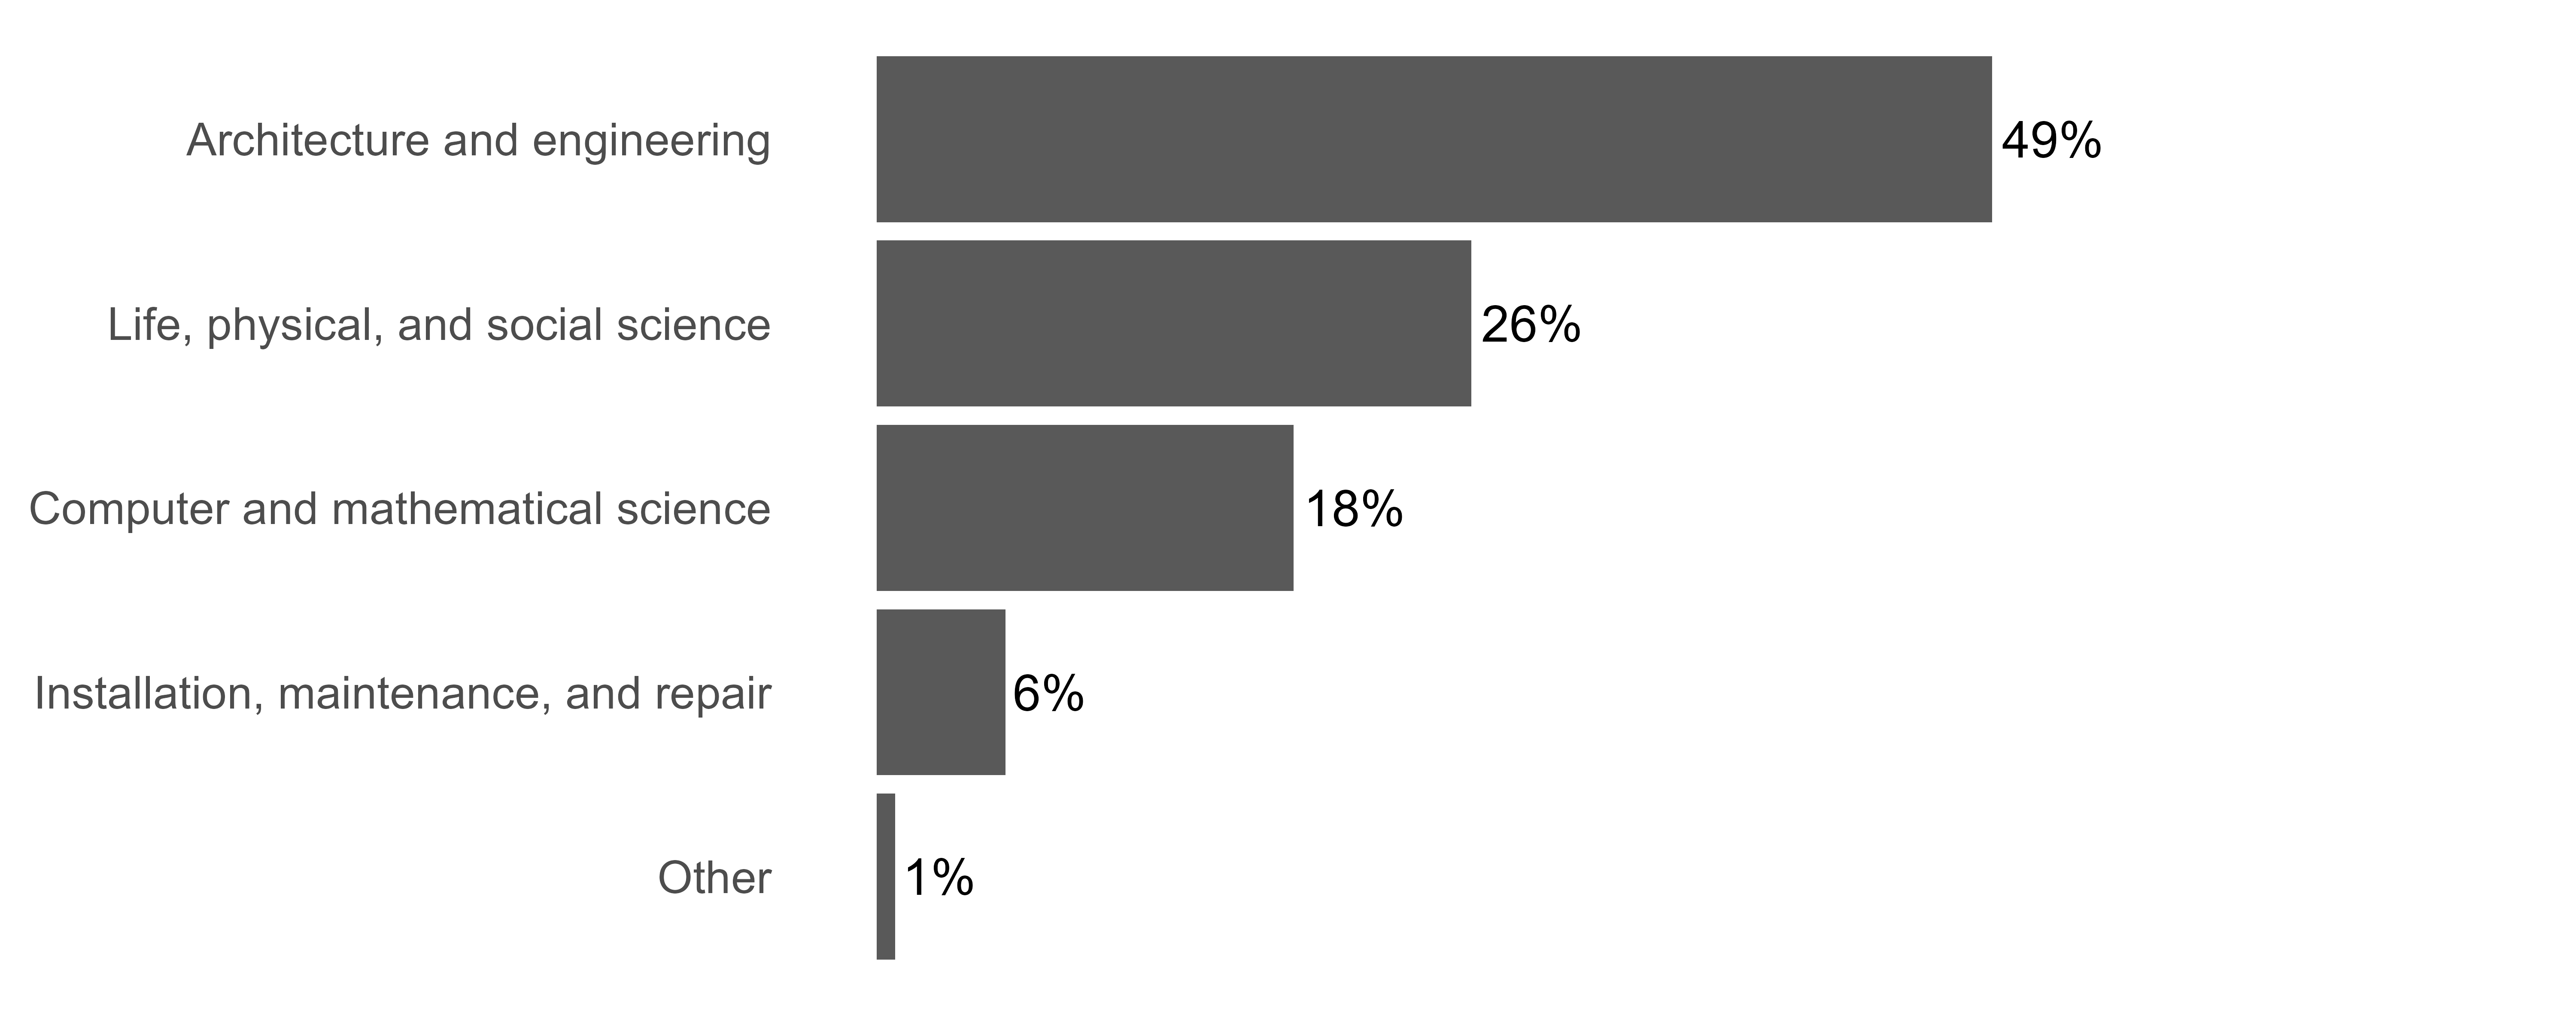
\includegraphics{outputs/figures/barplot_stem_cbos_stem_ocupacao.png}

}

\end{figure}%

\emph{Notes}: This figure shows the top five occupations among the 120
STEM mayors in our sample. Municipalities chosen were those that held
ordinary elections in selected years (2016, 2020) whose mayor was
elected in the first round and among the top two most voted was a STEM
candidate and a Non-STEM one.

\subsection{Percentage of municipalities with a STEM mayor among top 2
per
state}\label{percentage-of-municipalities-with-a-stem-mayor-among-top-2-per-state}

\begin{figure}[H]

\caption{Percentage of municipalities with a STEM mayor among top 2 per
state}

{\centering 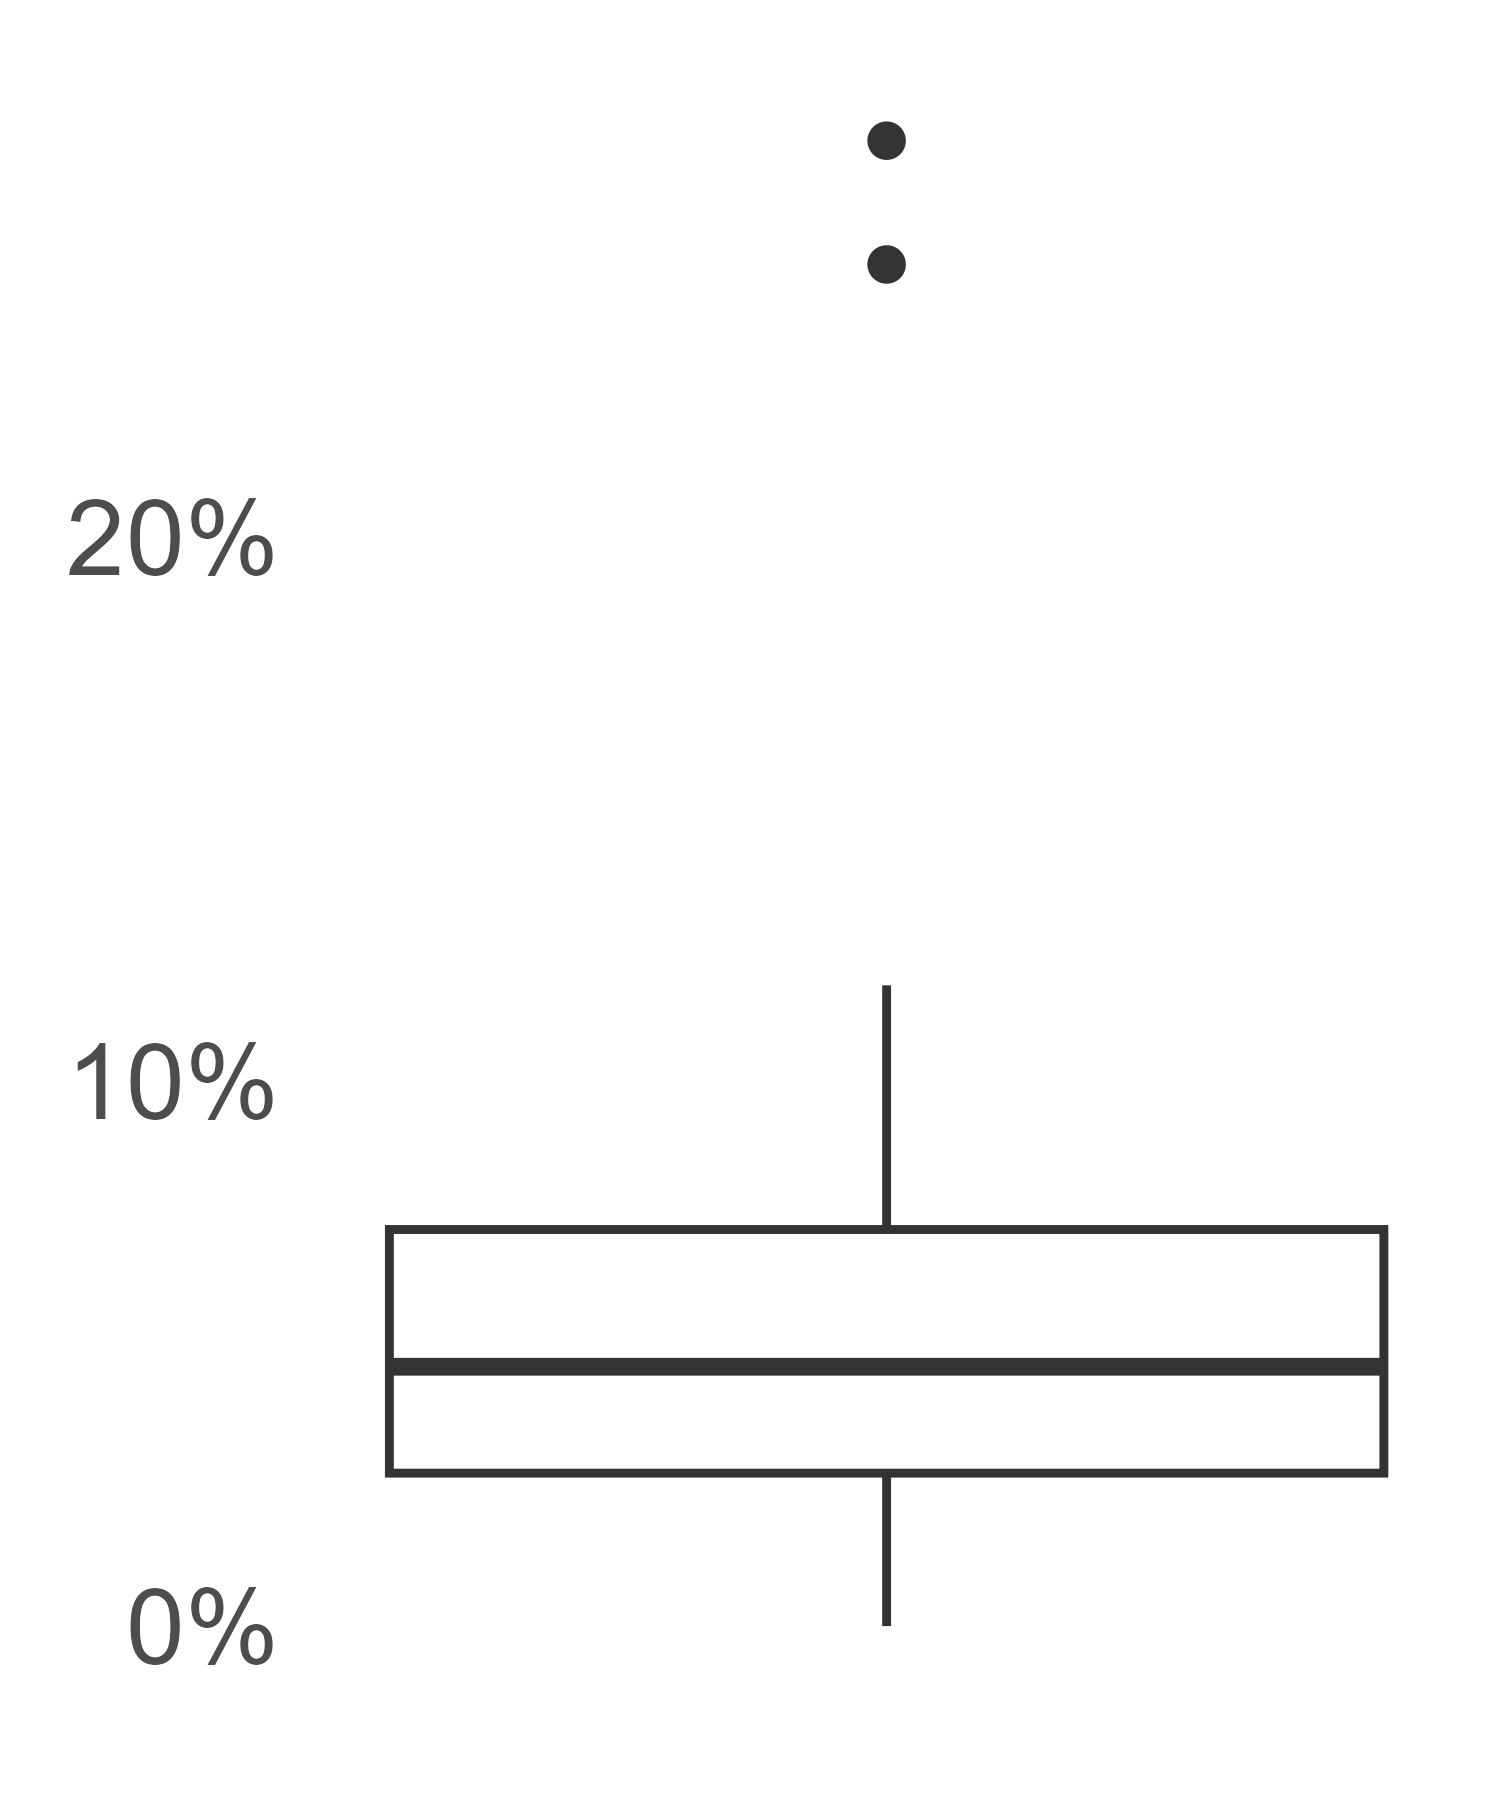
\includegraphics{outputs/figures/sumstats_boxplot.png}

}

\end{figure}%

\emph{Notes}: This plot shows the distribution per state of the
percentage of municipalities that had a STEM mayor among top 2 voted.
Municipalities chosen were those that held ordinary elections in
selected years (2016, 2020) whose mayor was elected in the first round
and among the top two most voted was a STEM candidate and a Non-STEM
one.

\subsection{Municipalities with a STEM candidate
(2016)}\label{municipalities-with-a-stem-candidate-2016}

\begin{figure}[H]

\caption{Municipalities with a STEM candidate (2016)}

{\centering 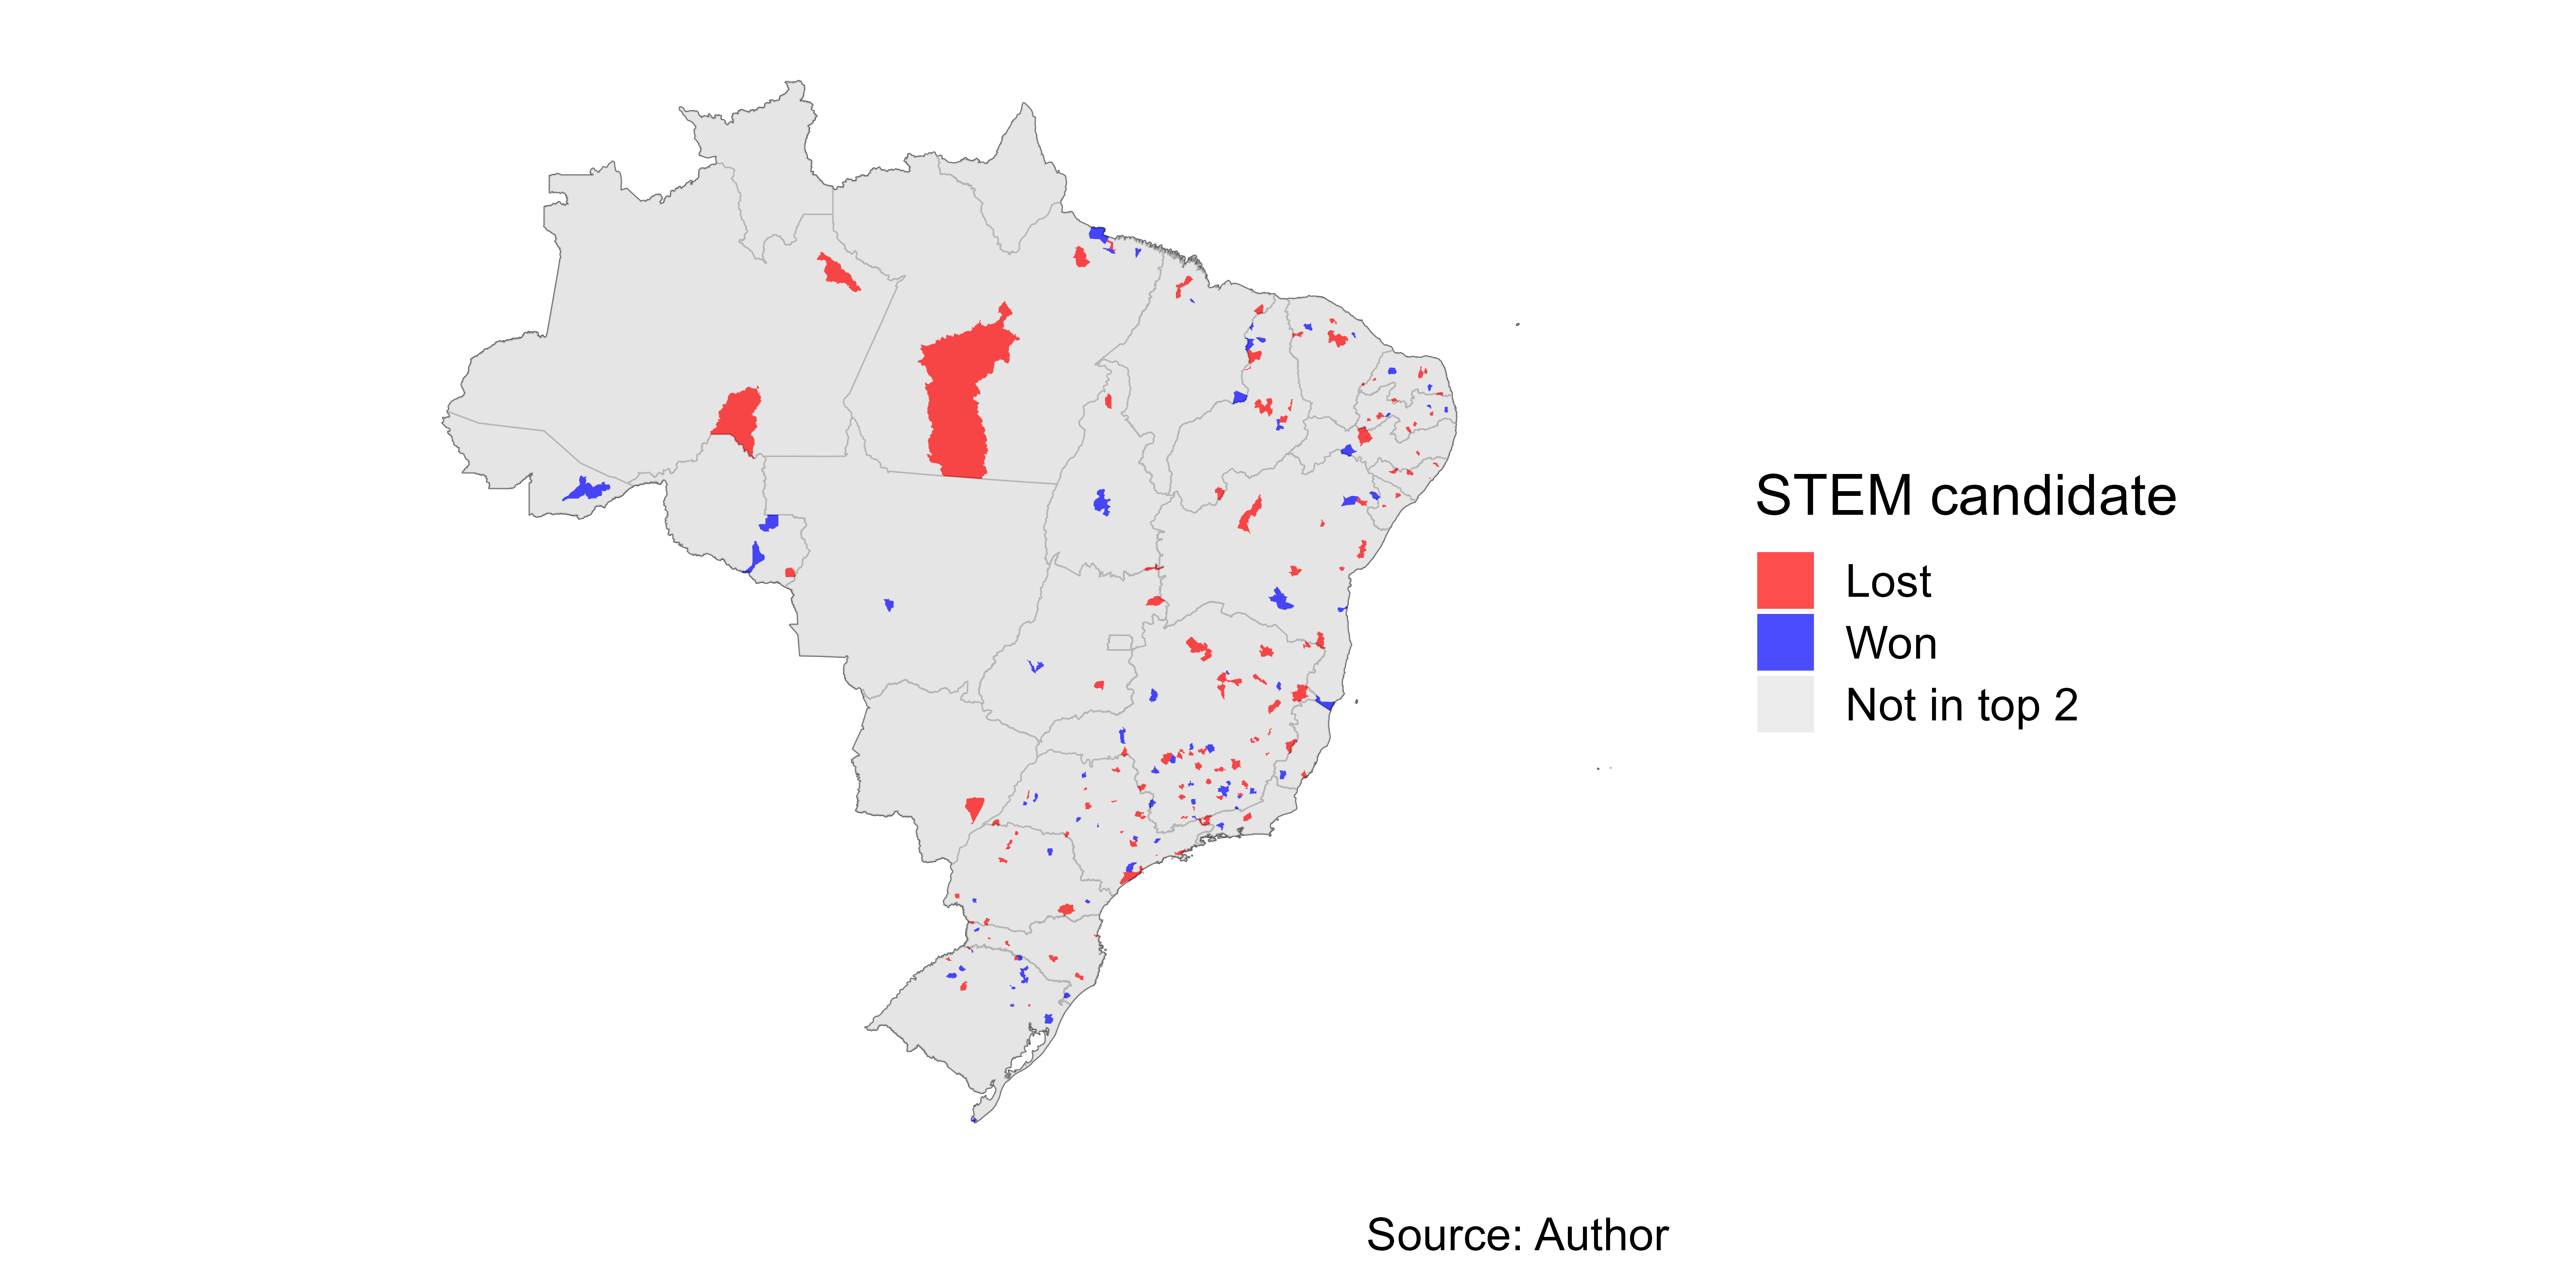
\includegraphics{outputs/figures/mapa_stem_municipios_2016.png}

}

\end{figure}%

\emph{Notes}: In this figure, we colored all municipalities in our 2016
sample, that is, where a STEM candidate was among the top two most
voted. In red are the municipalities where the STEM candidate lost and
in blue are the municipalities where the STEM candidate won. In gray are
all the municipalities with no STEM candidate among the top two most
voted.

\subsection{Impact of STEM mayor election on epidemiological
outcomes}\label{impact-of-stem-mayor-election-on-epidemiological-outcomes}

\begin{figure}[H]

\caption{Impact of STEM mayor election on epidemiological outcomes}

{\centering 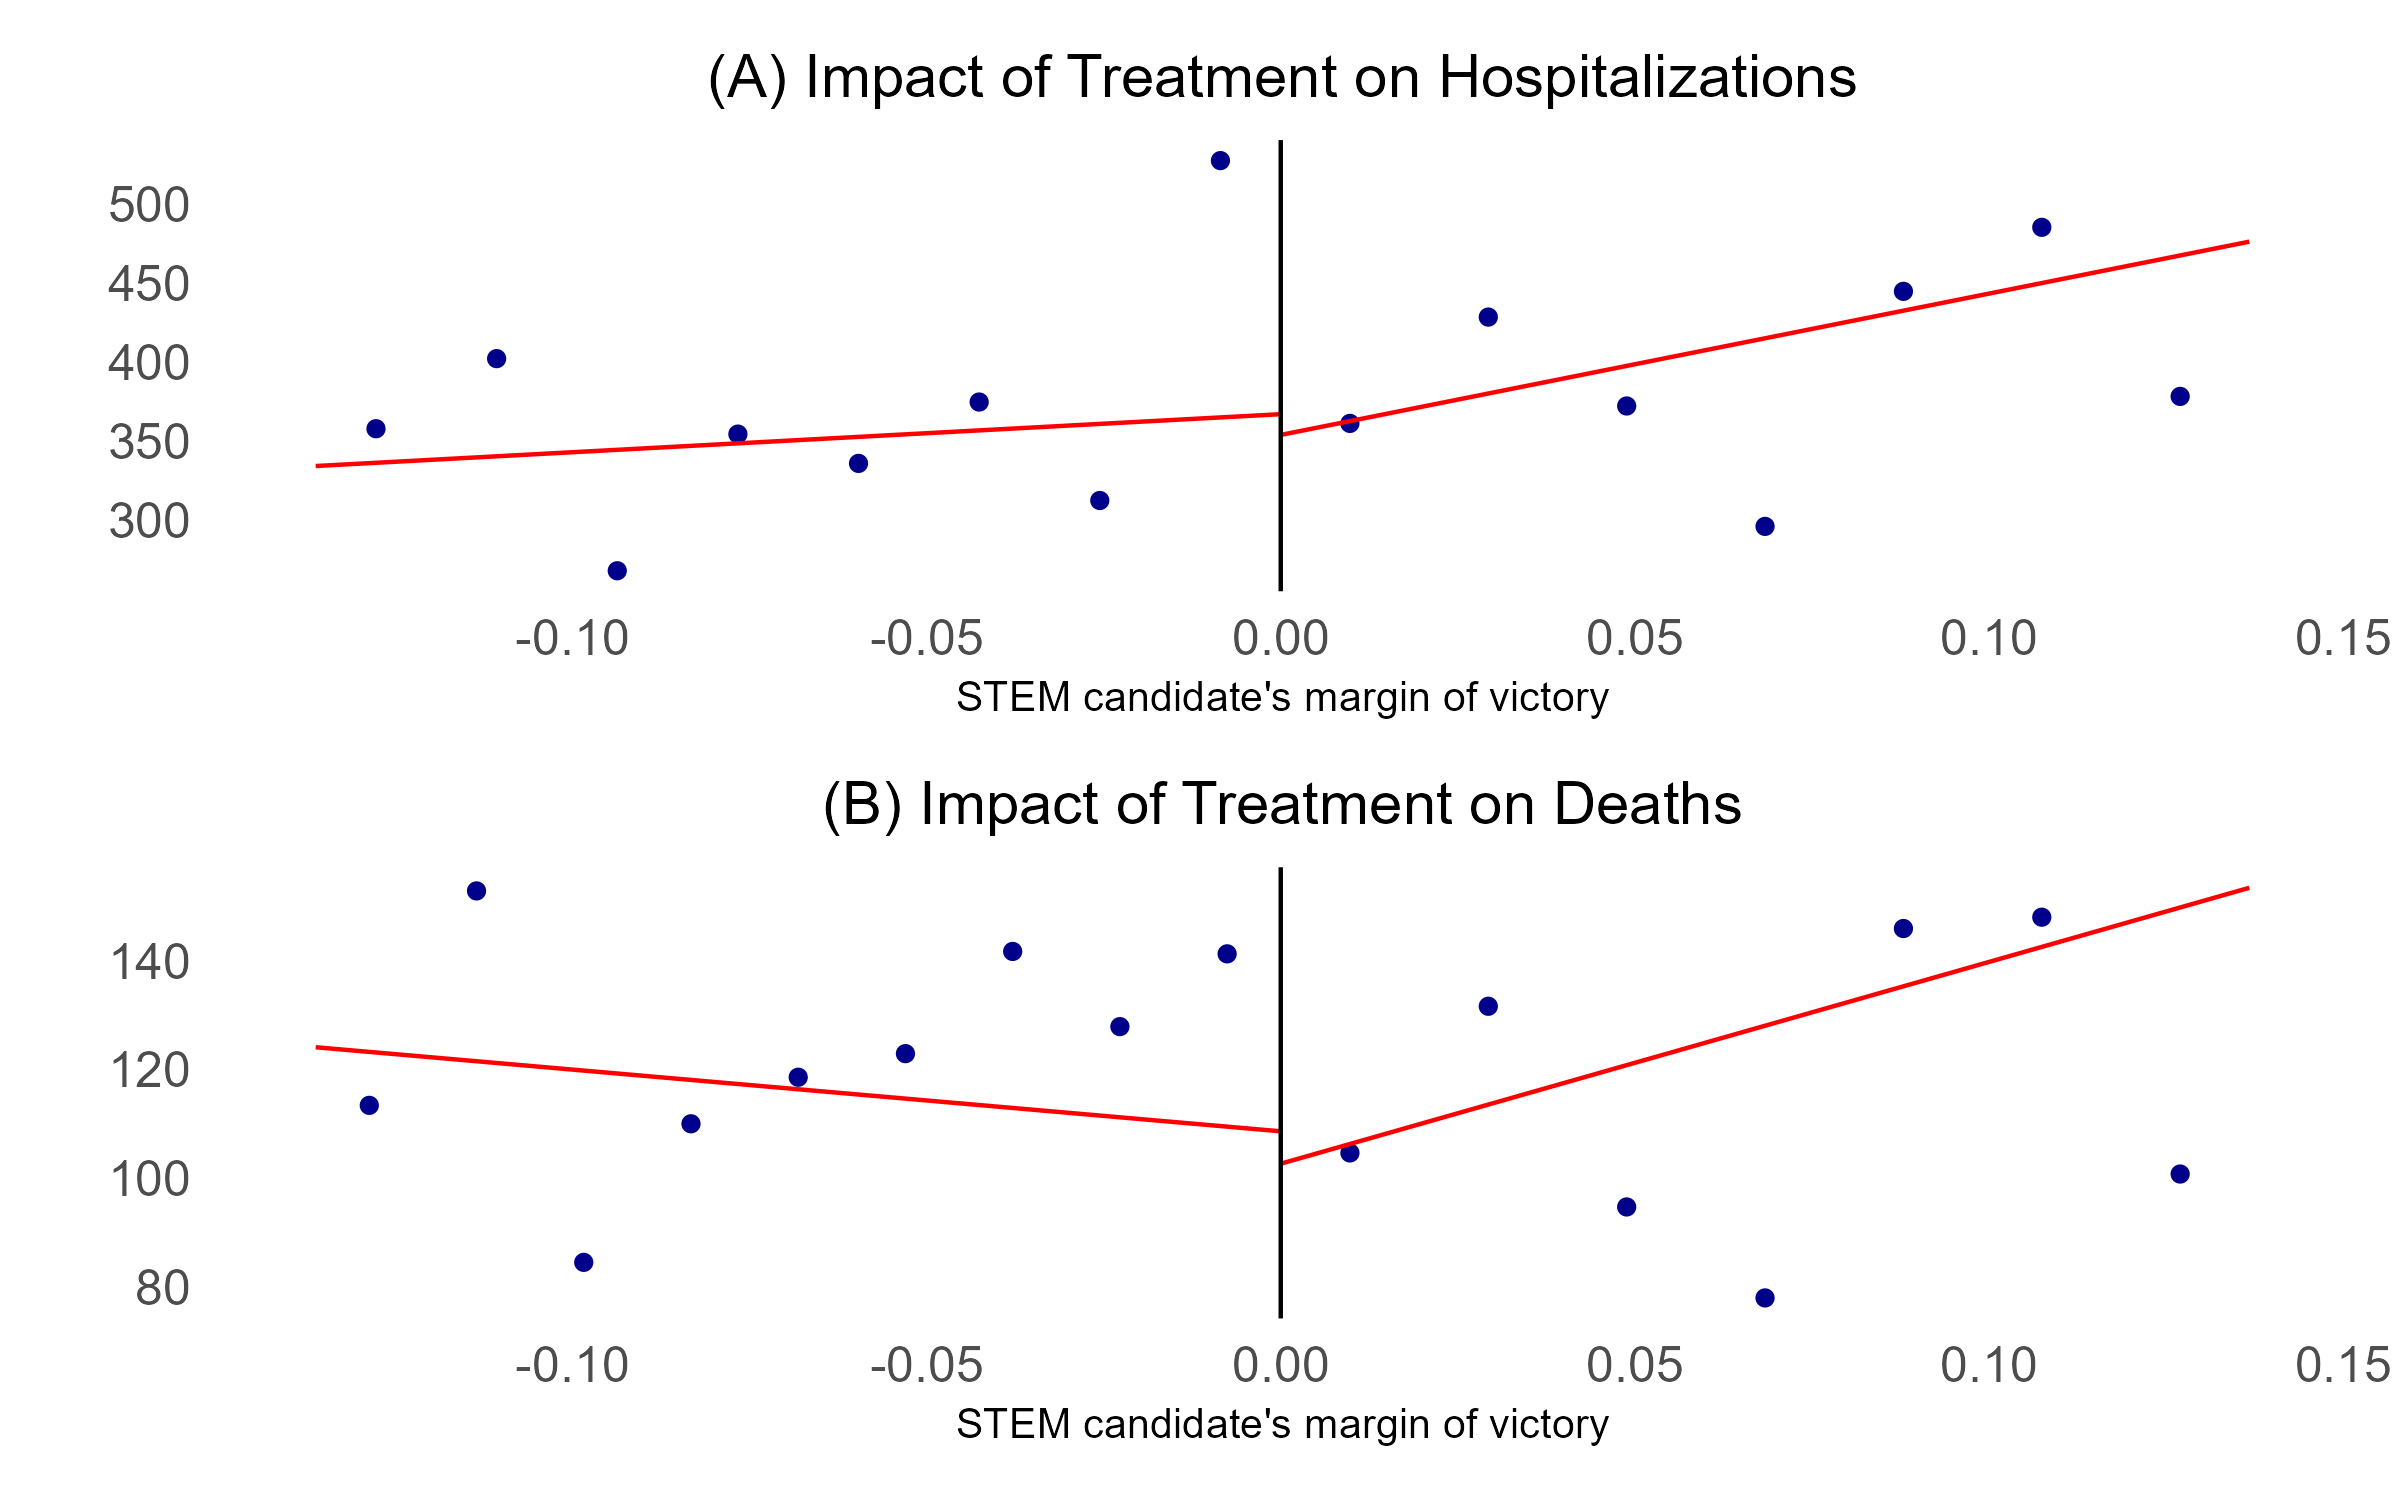
\includegraphics{outputs/figures/bigsample_plots_outcomes.png}

}

\end{figure}%

\emph{Notes}: This figure reports the RD estimated impact of mayors with
scientific background on deaths and hospitalizations by COVID-19 per
hundred thousand inhabitants. Municipalities chosen were those that held
ordinary elections in selected years (2016, 2020) whose mayor was
elected in the first round and among the top two most voted was a STEM
candidate and a Non-STEM one.

\subsection{Baseline Characteristics - RD Estimates
(Demographics)}\label{baseline-characteristics---rd-estimates-demographics}

\begin{longtable}[]{@{}
  >{\raggedright\arraybackslash}p{(\columnwidth - 10\tabcolsep) * \real{0.1829}}
  >{\raggedright\arraybackslash}p{(\columnwidth - 10\tabcolsep) * \real{0.1463}}
  >{\raggedright\arraybackslash}p{(\columnwidth - 10\tabcolsep) * \real{0.2073}}
  >{\raggedright\arraybackslash}p{(\columnwidth - 10\tabcolsep) * \real{0.1098}}
  >{\raggedright\arraybackslash}p{(\columnwidth - 10\tabcolsep) * \real{0.1341}}
  >{\raggedright\arraybackslash}p{(\columnwidth - 10\tabcolsep) * \real{0.1707}}@{}}
\caption{Baseline Characteristics - RD Estimates
(Demography)}\tabularnewline
\toprule\noalign{}
\begin{minipage}[b]{\linewidth}\raggedright
\end{minipage} & \begin{minipage}[b]{\linewidth}\raggedright
PC income
\end{minipage} & \begin{minipage}[b]{\linewidth}\raggedright
Log Population
\end{minipage} & \begin{minipage}[b]{\linewidth}\raggedright
HDI
\end{minipage} & \begin{minipage}[b]{\linewidth}\raggedright
Density
\end{minipage} & \begin{minipage}[b]{\linewidth}\raggedright
\% Masc. Pop
\end{minipage} \\
\midrule\noalign{}
\endfirsthead
\toprule\noalign{}
\begin{minipage}[b]{\linewidth}\raggedright
\end{minipage} & \begin{minipage}[b]{\linewidth}\raggedright
PC income
\end{minipage} & \begin{minipage}[b]{\linewidth}\raggedright
Log Population
\end{minipage} & \begin{minipage}[b]{\linewidth}\raggedright
HDI
\end{minipage} & \begin{minipage}[b]{\linewidth}\raggedright
Density
\end{minipage} & \begin{minipage}[b]{\linewidth}\raggedright
\% Masc. Pop
\end{minipage} \\
\midrule\noalign{}
\endhead
\bottomrule\noalign{}
\endlastfoot
RD estimator & 2.68 & 0.18 & 0.01 & 66.11 & 0.22 \\
& {[}7.32{]} & {[}0.49{]} & {[}0.01{]} & {[}103.90{]} & {[}0.74{]} \\
& 0.71 & 0.71 & 0.63 & 0.52 & 0.76 \\
Eff.N.obs. & 119 & 92 & 93 & 65 & 105 \\
Bandwidth & 15.25 & 10.98 & 11.31 & 7.69 & 13.98 \\
\end{longtable}

\emph{Notes}: This table reports the RD estimated impact of mayors with
scientific background on demographic baseline characteristics.
Municipalities chosen were those that held ordinary elections in
selected years (2016, 2020) whose mayor was elected in the first round
and among the top two most voted was a STEM candidate and a Non-STEM
one. All specifications use state fixed-effects, uniform kernel and
optimal bandwidths calculated following Calonico et al.~(2014). We
report robust-bias corrected p-values, conventional (non-robust)
estimates and standard errors.

\subsection{Baseline Characteristics - RD Estimates (Health and
Ideology)}\label{baseline-characteristics---rd-estimates-health-and-ideology}

\begin{longtable}[]{@{}
  >{\raggedright\arraybackslash}p{(\columnwidth - 10\tabcolsep) * \real{0.0974}}
  >{\raggedright\arraybackslash}p{(\columnwidth - 10\tabcolsep) * \real{0.1948}}
  >{\raggedright\arraybackslash}p{(\columnwidth - 10\tabcolsep) * \real{0.1429}}
  >{\raggedright\arraybackslash}p{(\columnwidth - 10\tabcolsep) * \real{0.2208}}
  >{\raggedright\arraybackslash}p{(\columnwidth - 10\tabcolsep) * \real{0.1753}}
  >{\raggedright\arraybackslash}p{(\columnwidth - 10\tabcolsep) * \real{0.1429}}@{}}
\caption{Baseline Characteristics - RD Estimates (Health and
Ideology)}\tabularnewline
\toprule\noalign{}
\begin{minipage}[b]{\linewidth}\raggedright
\end{minipage} & \begin{minipage}[b]{\linewidth}\raggedright
\% Health municipal spending
\end{minipage} & \begin{minipage}[b]{\linewidth}\raggedright
Doctors per 1k pop.
\end{minipage} & \begin{minipage}[b]{\linewidth}\raggedright
Community health agents program
\end{minipage} & \begin{minipage}[b]{\linewidth}\raggedright
Hosp. beds per 100k pop.
\end{minipage} & \begin{minipage}[b]{\linewidth}\raggedright
Mun. ideology index
\end{minipage} \\
\midrule\noalign{}
\endfirsthead
\toprule\noalign{}
\begin{minipage}[b]{\linewidth}\raggedright
\end{minipage} & \begin{minipage}[b]{\linewidth}\raggedright
\% Health municipal spending
\end{minipage} & \begin{minipage}[b]{\linewidth}\raggedright
Doctors per 1k pop.
\end{minipage} & \begin{minipage}[b]{\linewidth}\raggedright
Community health agents program
\end{minipage} & \begin{minipage}[b]{\linewidth}\raggedright
Hosp. beds per 100k pop.
\end{minipage} & \begin{minipage}[b]{\linewidth}\raggedright
Mun. ideology index
\end{minipage} \\
\midrule\noalign{}
\endhead
\bottomrule\noalign{}
\endlastfoot
RD estimator & 4.42 & -0.17 & -5.79 & -28.47 & 0.07 \\
& {[}1.92{]} & {[}0.20{]} & {[}12.67{]} & {[}40.04{]} & {[}0.05{]} \\
& 0.02** & 0.40 & 0.65 & 0.48 & 0.16 \\
Eff.N.obs. & 104 & 69 & 95 & 96 & 76 \\
Bandwidth & 13.81 & 8.14 & 11.68 & 11.98 & 8.9 \\
\end{longtable}

\emph{Notes}: This table reports the RD estimated impact of mayors with
scientific background on health and ideology baseline characteristics.
Municipalities chosen were those that held ordinary elections in
selected years (2016, 2020) whose mayor was elected in the first round
and among the top two most voted was a STEM candidate and a Non-STEM
one. All specifications use state fixed-effects, uniform kernel and
optimal bandwidths calculated following Calonico et al.~(2014). The
ideology column regards mayors' party ideology, whereas negative numbers
represent left-wing parties and positive right-wing (Power \&
Rodrigues-Silveira, 2019).We report robust-bias corrected p-values,
estimates and standard errors.

\subsection{Impact of STEM Leadership on Epidemiological Outcomes --- RD
estimates}\label{impact-of-stem-leadership-on-epidemiological-outcomes-rd-estimates}

\begin{longtable}[]{@{}
  >{\raggedright\arraybackslash}p{(\columnwidth - 8\tabcolsep) * \real{0.2083}}
  >{\raggedright\arraybackslash}p{(\columnwidth - 8\tabcolsep) * \real{0.1528}}
  >{\raggedright\arraybackslash}p{(\columnwidth - 8\tabcolsep) * \real{0.1528}}
  >{\raggedright\arraybackslash}p{(\columnwidth - 8\tabcolsep) * \real{0.1389}}
  >{\raggedright\arraybackslash}p{(\columnwidth - 8\tabcolsep) * \real{0.1389}}@{}}
\caption{Impact of STEM Leadership on Epidemiological Outcomes --- RD
estimates}\tabularnewline
\toprule\noalign{}
\begin{minipage}[b]{\linewidth}\raggedright
\end{minipage} & \begin{minipage}[b]{\linewidth}\raggedright
\begin{enumerate}
\def\labelenumi{(\arabic{enumi})}
\tightlist
\item
\end{enumerate}
\end{minipage} & \begin{minipage}[b]{\linewidth}\raggedright
\begin{enumerate}
\def\labelenumi{(\arabic{enumi})}
\setcounter{enumi}{1}
\tightlist
\item
\end{enumerate}
\end{minipage} & \begin{minipage}[b]{\linewidth}\raggedright
\begin{enumerate}
\def\labelenumi{(\arabic{enumi})}
\setcounter{enumi}{2}
\tightlist
\item
\end{enumerate}
\end{minipage} & \begin{minipage}[b]{\linewidth}\raggedright
\begin{enumerate}
\def\labelenumi{(\arabic{enumi})}
\setcounter{enumi}{3}
\tightlist
\item
\end{enumerate}
\end{minipage} \\
\midrule\noalign{}
\endfirsthead
\toprule\noalign{}
\begin{minipage}[b]{\linewidth}\raggedright
\end{minipage} & \begin{minipage}[b]{\linewidth}\raggedright
\begin{enumerate}
\def\labelenumi{(\arabic{enumi})}
\tightlist
\item
\end{enumerate}
\end{minipage} & \begin{minipage}[b]{\linewidth}\raggedright
\begin{enumerate}
\def\labelenumi{(\arabic{enumi})}
\setcounter{enumi}{1}
\tightlist
\item
\end{enumerate}
\end{minipage} & \begin{minipage}[b]{\linewidth}\raggedright
\begin{enumerate}
\def\labelenumi{(\arabic{enumi})}
\setcounter{enumi}{2}
\tightlist
\item
\end{enumerate}
\end{minipage} & \begin{minipage}[b]{\linewidth}\raggedright
\begin{enumerate}
\def\labelenumi{(\arabic{enumi})}
\setcounter{enumi}{3}
\tightlist
\item
\end{enumerate}
\end{minipage} \\
\midrule\noalign{}
\endhead
\bottomrule\noalign{}
\endlastfoot
\multicolumn{5}{@{}>{\raggedright\arraybackslash}p{(\columnwidth - 8\tabcolsep) * \real{0.7917} + 8\tabcolsep}@{}}{%
Panel A: Deaths} \\
RD estimator & -32.36 & -26.73 & -54.85 & -48.93 \\
& {[}35.69{]} & {[}34.27{]} & {[}29.19{]} & {[}24.16{]} \\
& 0.36 & 0.44 & 0.06* & 0.04** \\
Eff.N.obs. & 117 & 117 & 119 & 65 \\
Bandwidth & 15 & 15 & 15.28 & 7.35 \\
\multicolumn{5}{@{}>{\raggedright\arraybackslash}p{(\columnwidth - 8\tabcolsep) * \real{0.7917} + 8\tabcolsep}@{}}{%
Panel B: Hospitalizations} \\
RD estimator & -114.66 & -142.69 & -47.67 & -115.47 \\
& {[}140.27{]} & {[}138.68{]} & {[}98.80{]} & {[}97.94{]} \\
& 0.41 & 0.30 & 0.63 & 0.24 \\
Eff.N.obs. & 117 & 117 & 110 & 78 \\
Bandwidth & 15 & 15 & 14.35 & 9.06 \\
\end{longtable}

\emph{Notes}: This table reports the RD estimated impact of mayors with
scientific background on deaths and hospitalizations by COVID-19 per
hundred thousand inhabitants. Municipalities chosen were those that held
ordinary elections in selected years (2016, 2020) whose mayor was
elected in the first round and among the top two most voted was a STEM
candidate and a Non-STEM one. All specifications use state
fixed-effects, uniform kernel. Estimations (3) and (4) use optimal
bandwidths calculated following Calonico et al.~(2014), while
estimations (1) and (2) use a 0.15\% vote margin difference between the
two most voted candidates, in order to best understand the inclusion of
covariates. Estimations (2) and (4) control for mayors' personal
characteristics. We report robust-bias-corrected p-values, coefficients
and standard errors.

\subsection{STEM candidates' personal characteristics --- RD
estimates}\label{stem-candidates-personal-characteristics-rd-estimates}

\begin{longtable}[]{@{}
  >{\raggedright\arraybackslash}p{(\columnwidth - 8\tabcolsep) * \real{0.2055}}
  >{\raggedright\arraybackslash}p{(\columnwidth - 8\tabcolsep) * \real{0.1233}}
  >{\raggedright\arraybackslash}p{(\columnwidth - 8\tabcolsep) * \real{0.1644}}
  >{\raggedright\arraybackslash}p{(\columnwidth - 8\tabcolsep) * \real{0.1233}}
  >{\raggedright\arraybackslash}p{(\columnwidth - 8\tabcolsep) * \real{0.3425}}@{}}
\caption{STEM candidates' personal characteristics --- RD
estimates}\tabularnewline
\toprule\noalign{}
\begin{minipage}[b]{\linewidth}\raggedright
\end{minipage} & \begin{minipage}[b]{\linewidth}\raggedright
Women
\end{minipage} & \begin{minipage}[b]{\linewidth}\raggedright
Incumbent
\end{minipage} & \begin{minipage}[b]{\linewidth}\raggedright
Age
\end{minipage} & \begin{minipage}[b]{\linewidth}\raggedright
Mayors' party ideology
\end{minipage} \\
\midrule\noalign{}
\endfirsthead
\toprule\noalign{}
\begin{minipage}[b]{\linewidth}\raggedright
\end{minipage} & \begin{minipage}[b]{\linewidth}\raggedright
Women
\end{minipage} & \begin{minipage}[b]{\linewidth}\raggedright
Incumbent
\end{minipage} & \begin{minipage}[b]{\linewidth}\raggedright
Age
\end{minipage} & \begin{minipage}[b]{\linewidth}\raggedright
Mayors' party ideology
\end{minipage} \\
\midrule\noalign{}
\endhead
\bottomrule\noalign{}
\endlastfoot
RD estimator & -0.13 & 0.17 & 3.49 & 0.10 \\
& {[}0.06{]} & {[}0.15{]} & {[}4.84{]} & {[}0.13{]} \\
& 0.04** & 0.25 & 0.47 & 0.43 \\
Eff.N.obs. & 89 & 82 & 82 & 104 \\
Bandwidth & 10.43 & 9.48 & 9.64 & 13.96 \\
\end{longtable}

\emph{Notes}: This table reports our RD estimates of the association
between STEM mayors and four outcomes. In the first column, we see the
effect on mayors' personal characteristics. In the second column, the
measure of mayors were incumbents. The third column measures the effect
of mayors' age. The fourth column regards mayors' party ideology,
whereas negative numbers represent left-wing parties and positive
right-wing (Power \& Rodrigues-Silveira, 2019). All specifications use
state fixed-effects, uniform kernels. Optimal bandwidths were calculated
following Calonico et al.~(2014). We report robust-bias corrected
p-values, estimates and standard errors.

\subsection{Impact of STEM Candidate Elected in 2016 on
Non-Pharmaceutical
Interventions}\label{impact-of-stem-candidate-elected-in-2016-on-non-pharmaceutical-interventions}

\begin{longtable}[]{@{}
  >{\raggedright\arraybackslash}p{(\columnwidth - 12\tabcolsep) * \real{0.1083}}
  >{\raggedright\arraybackslash}p{(\columnwidth - 12\tabcolsep) * \real{0.1000}}
  >{\raggedright\arraybackslash}p{(\columnwidth - 12\tabcolsep) * \real{0.0750}}
  >{\raggedright\arraybackslash}p{(\columnwidth - 12\tabcolsep) * \real{0.1667}}
  >{\raggedright\arraybackslash}p{(\columnwidth - 12\tabcolsep) * \real{0.1833}}
  >{\raggedright\arraybackslash}p{(\columnwidth - 12\tabcolsep) * \real{0.1917}}
  >{\raggedright\arraybackslash}p{(\columnwidth - 12\tabcolsep) * \real{0.1333}}@{}}
\caption{Impact of STEM Candidate Elected in 2016 on Non-Pharmaceutical
Interventions in 2020}\tabularnewline
\toprule\noalign{}
\begin{minipage}[b]{\linewidth}\raggedright
\end{minipage} & \begin{minipage}[b]{\linewidth}\raggedright
Total NFI
\end{minipage} & \begin{minipage}[b]{\linewidth}\raggedright
Masks
\end{minipage} & \begin{minipage}[b]{\linewidth}\raggedright
Restrictions atv.
\end{minipage} & \begin{minipage}[b]{\linewidth}\raggedright
Restrictions circu.
\end{minipage} & \begin{minipage}[b]{\linewidth}\raggedright
Restrictions transp.
\end{minipage} & \begin{minipage}[b]{\linewidth}\raggedright
Sani barriers
\end{minipage} \\
\midrule\noalign{}
\endfirsthead
\toprule\noalign{}
\begin{minipage}[b]{\linewidth}\raggedright
\end{minipage} & \begin{minipage}[b]{\linewidth}\raggedright
Total NFI
\end{minipage} & \begin{minipage}[b]{\linewidth}\raggedright
Masks
\end{minipage} & \begin{minipage}[b]{\linewidth}\raggedright
Restrictions atv.
\end{minipage} & \begin{minipage}[b]{\linewidth}\raggedright
Restrictions circu.
\end{minipage} & \begin{minipage}[b]{\linewidth}\raggedright
Restrictions transp.
\end{minipage} & \begin{minipage}[b]{\linewidth}\raggedright
Sani barriers
\end{minipage} \\
\midrule\noalign{}
\endhead
\bottomrule\noalign{}
\endlastfoot
Robust & -20.56 & 0.55 & -0.02 & 0.75 & 0.82 & -0.47 \\
& {[}17.84{]} & {[}2.61{]} & {[}0.33{]} & {[}0.46{]} & {[}0.28{]} &
{[}0.22{]} \\
& 0.25 & 0.83 & 0.94 & 0.11 & \textless0.01*** & 0.03** \\
Eff.N.obs. & 8 & 18 & 10 & 28 & 25 & 10 \\
Bandwidth & 2.5 & 5.58 & 3.65 & 10.25 & 9.73 & 2.52 \\
\end{longtable}

\emph{Notes}: This figure reports the RD estimated impact of mayors with
scientific background on the adoption of non-pharmaceutical
interventions (NPIs) in 2020. Municipalities chosen were those that held
ordinary elections in 2016 whose mayor was elected in the first round
and among the top two most voted was a STEM candidate and a Non-STEM
one. All specifications use state fixed-effects, uniform kernel and
optimal bandwidths calculated following Calonico et al.~(2014).
Following the order of the columns, the interventions are: total number
of NPIs, face-covering restrictions, non-essential activities
restrictions, public gathering restrictions, public transport
restrictions and cordon sanitaire restrictions (the control of people
entering and leaving the city), as published by de Souza Santos et
al.~(2021). All specifications use state fixed-effects and triangular
kernels and control for mayors' age. We report robust-bias corrected
p-values, estimates and standard errors.

\subsection{Impact of STEM mayor on epidemiological outcomes using
different
bandwidths}\label{impact-of-stem-mayor-on-epidemiological-outcomes-using-different-bandwidths}

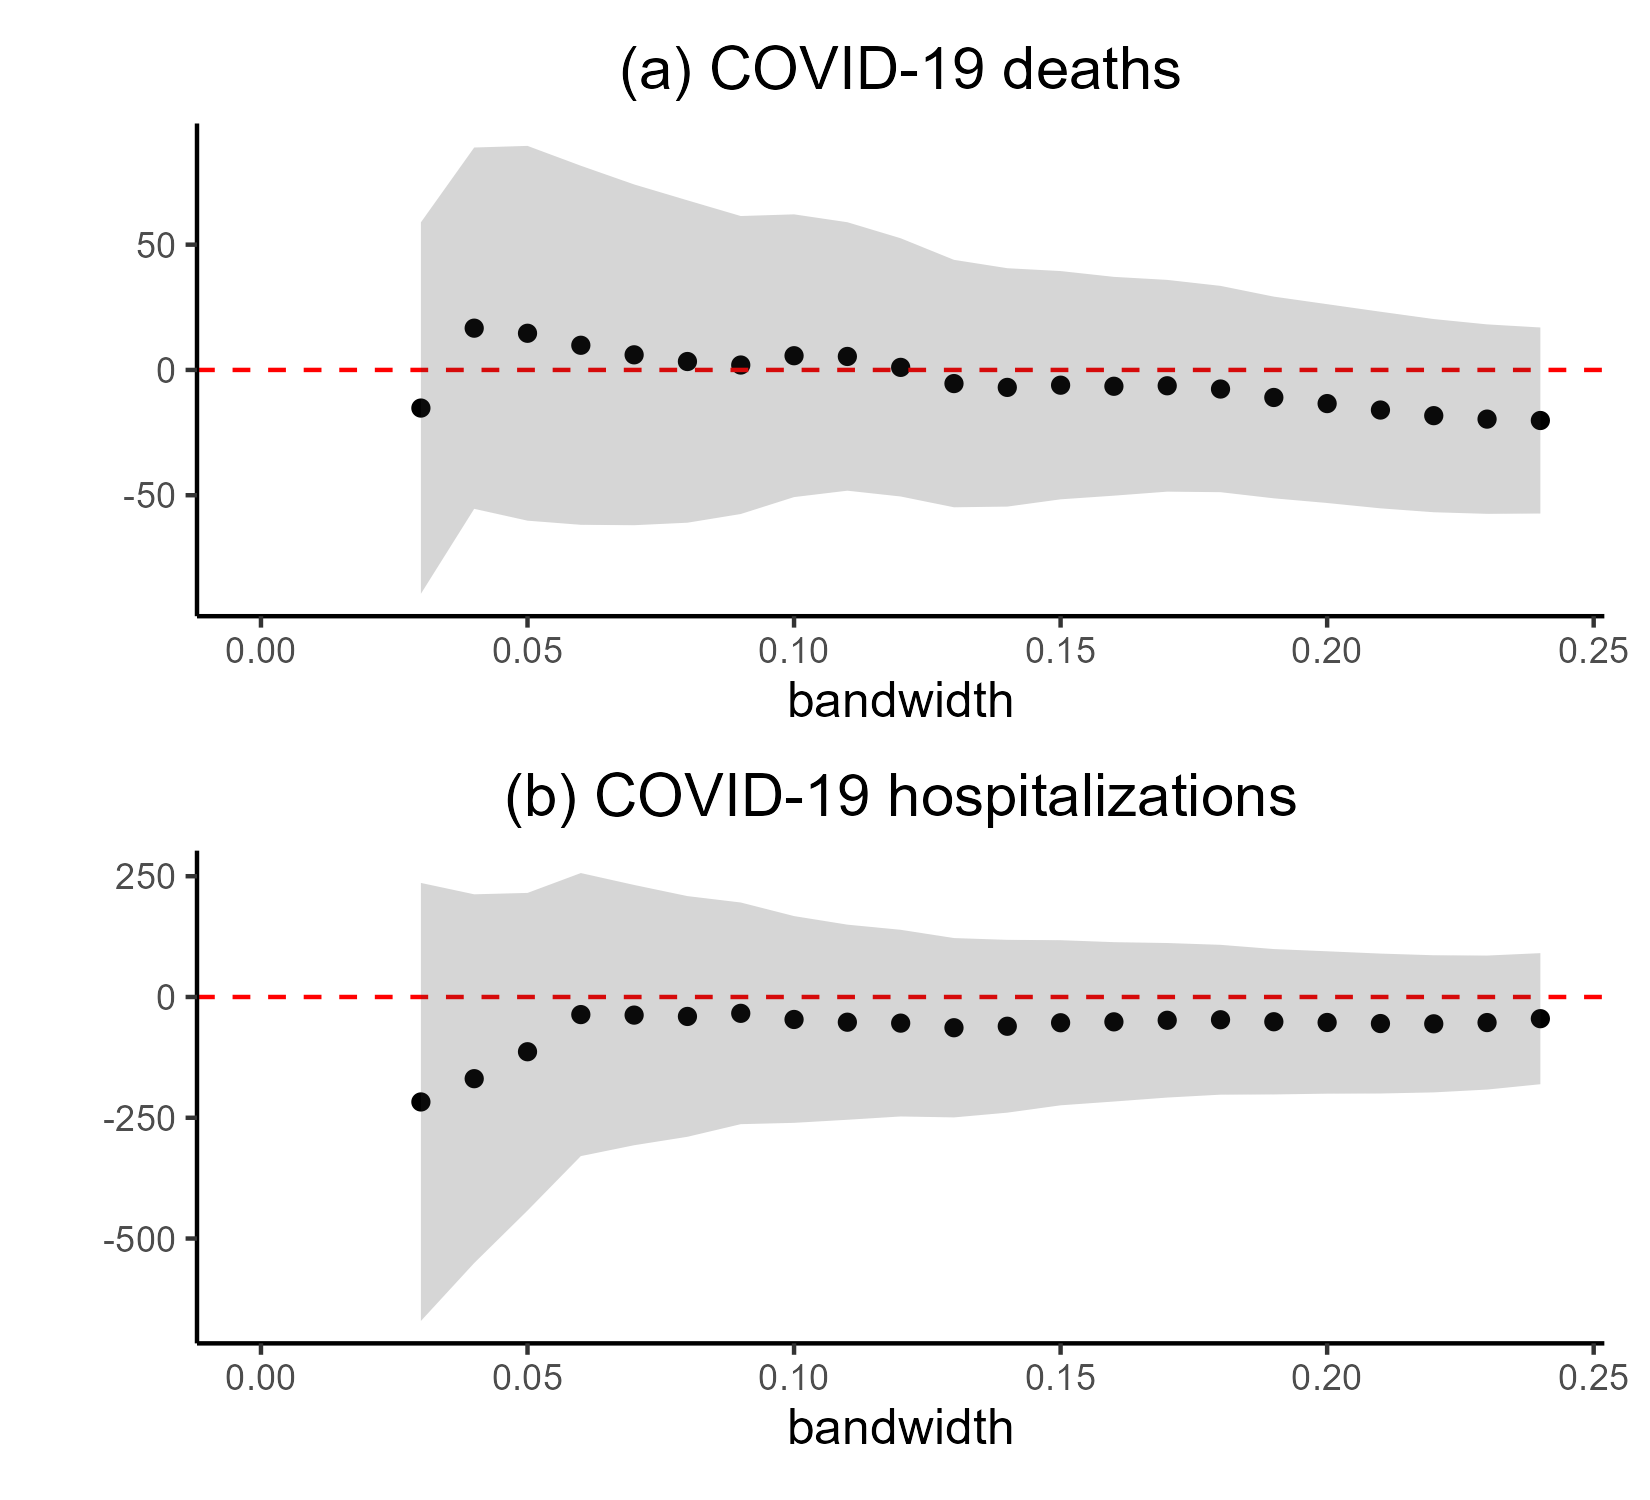
\includegraphics{outputs/figures/robust_outcomes.png} \emph{Notes}: This
figure reports the RD estimated impact of mayors with scientific
background on deaths and hospitalizations by COVID-19 per hundred
thousand inhabitants. Municipalities chosen were those that held
ordinary elections in selected years (2016, 2020) whose mayor was
elected in the first round and among the top two most voted was a STEM
candidate and a Non-STEM one. In the horizontal axis, we test different
winning margins (bandwidth) between the elected mayor and the second
most voted. These results represent the impact of our main estimation
(2) that uses first-degree polynomial, state fixed-effects, uniform
kernel, and control for mayors' personal characteristics.

\subsection{Impact of STEM mayor on non-pharmaceutical interventions
(NPIs) using different
bandwidths}\label{impact-of-stem-mayor-on-non-pharmaceutical-interventions-npis-using-different-bandwidths}

\begin{figure}[H]

\caption{Impact of STEM mayor on non-pharmaceutical interventions (NPIs)
using different bandwidths}

{\centering 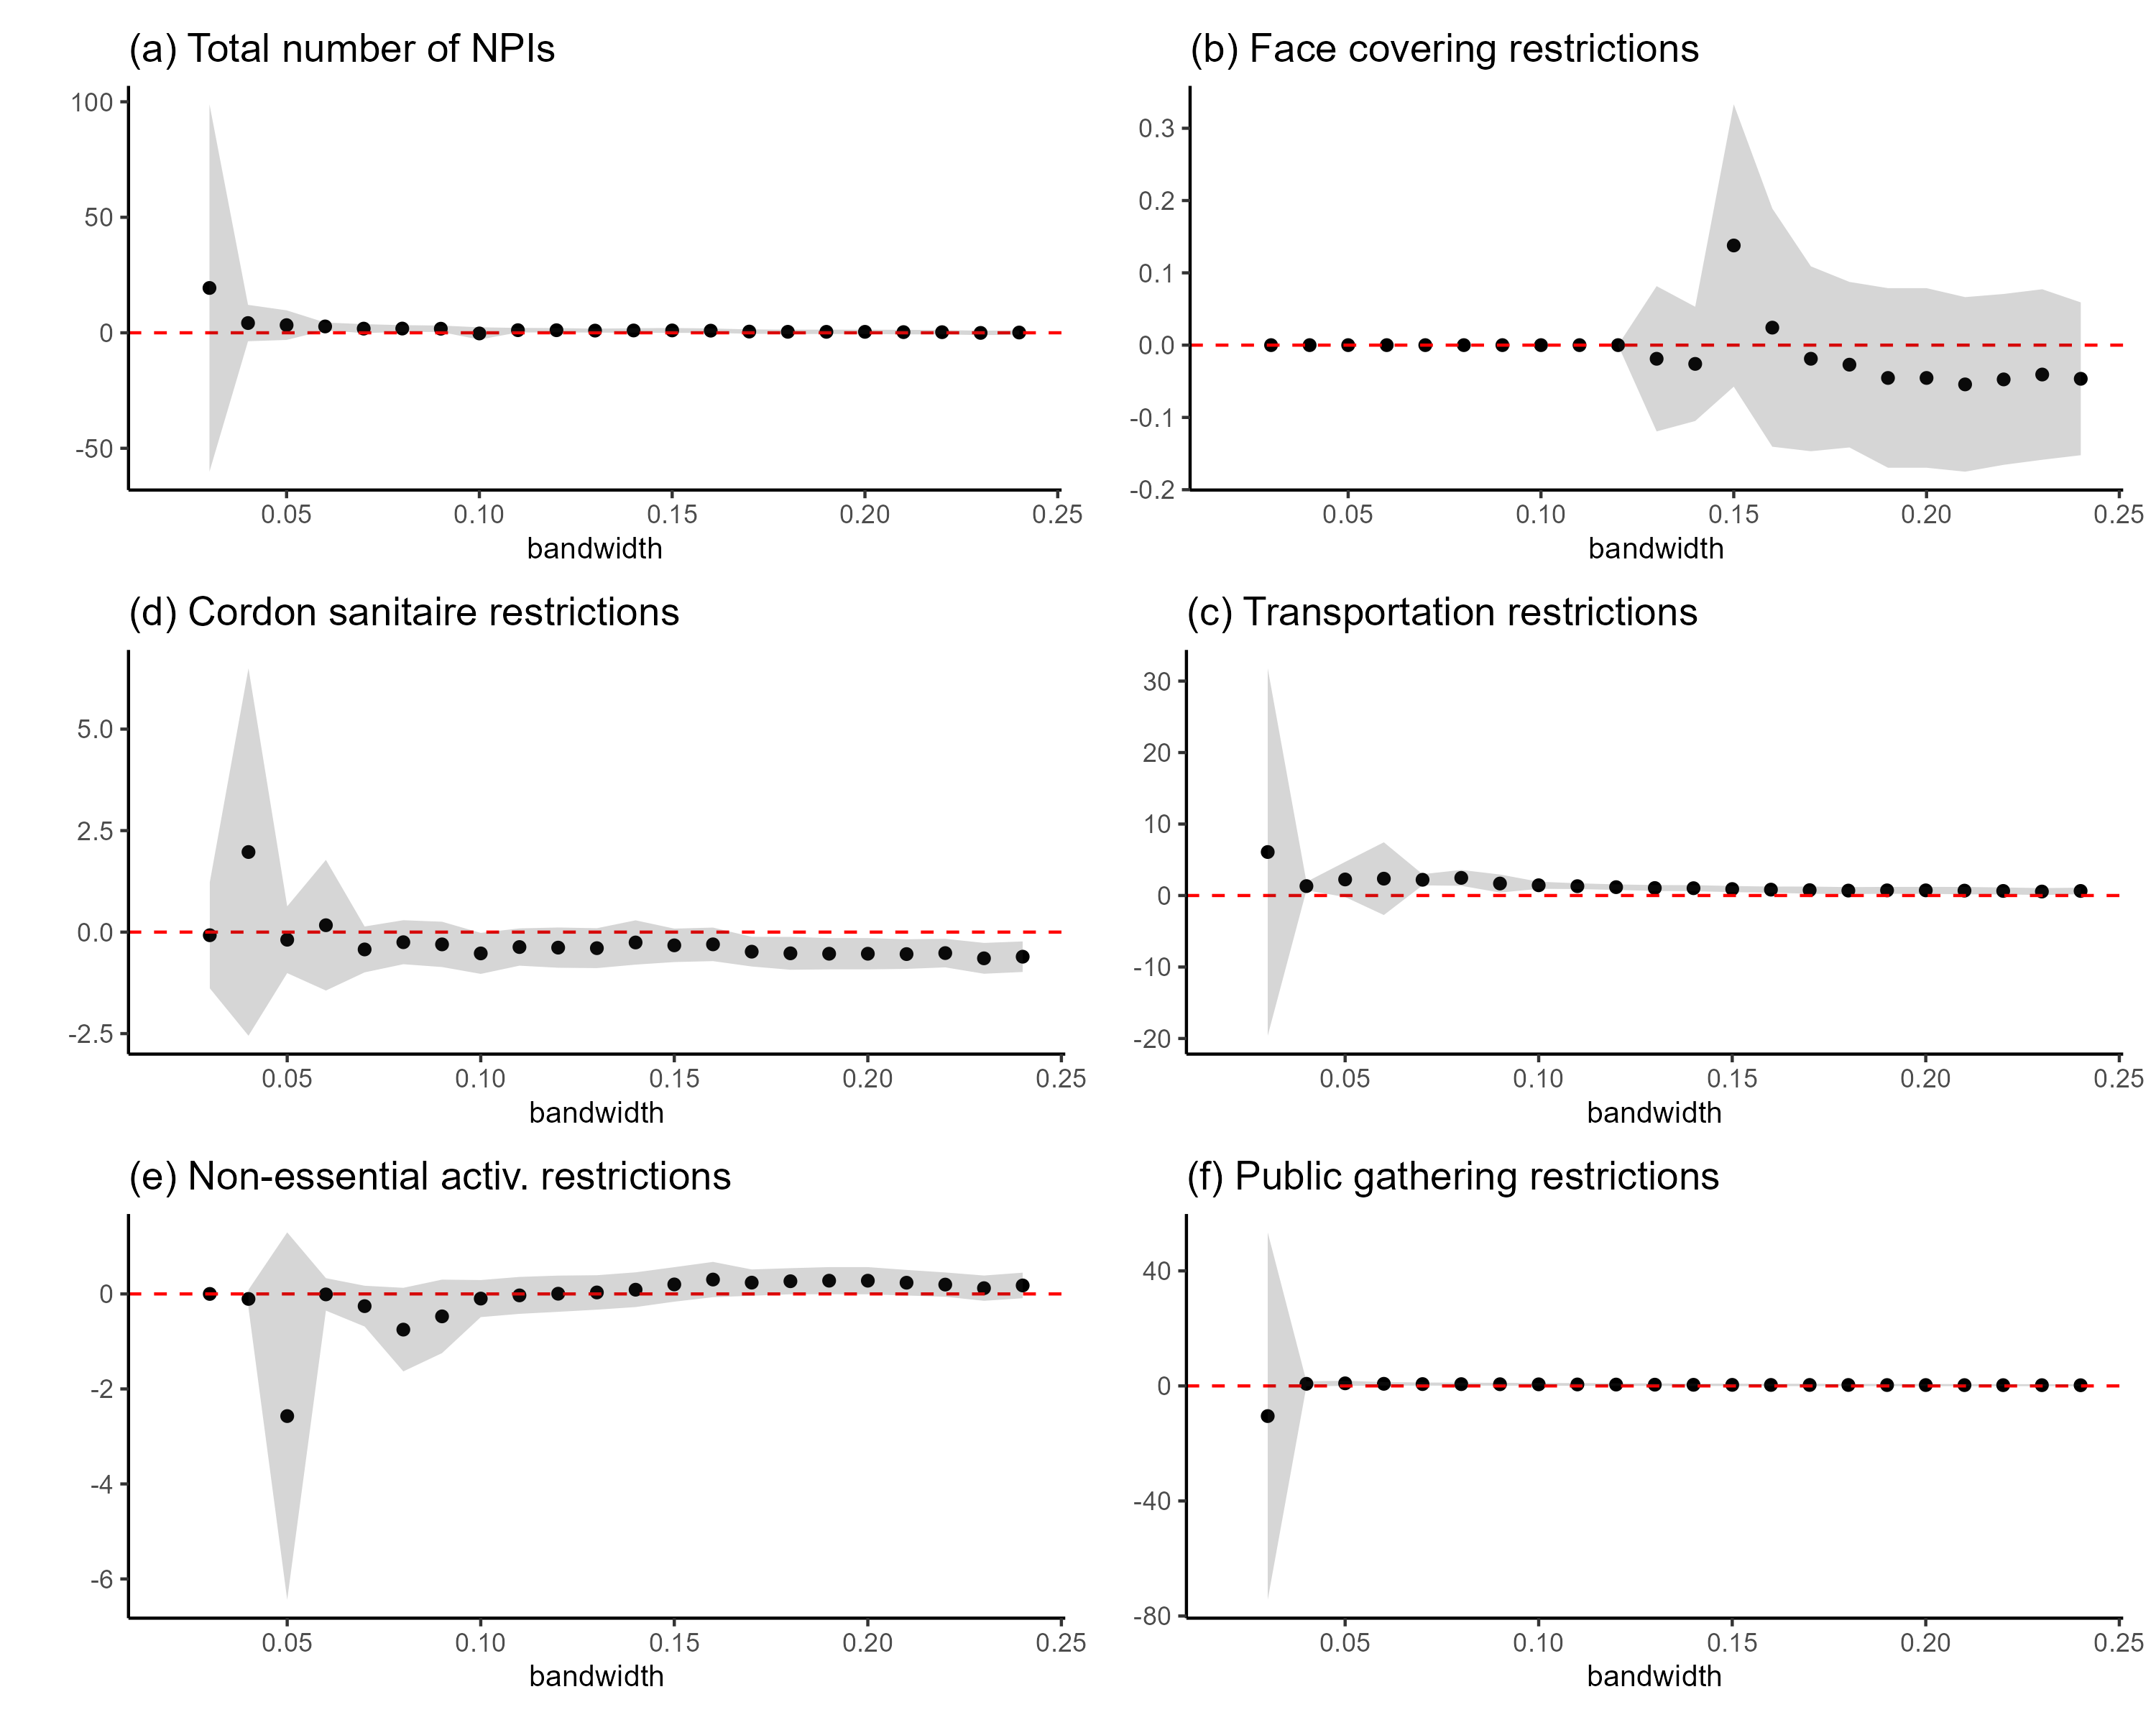
\includegraphics{outputs/figures/npi_rob.png}

}

\end{figure}%

\emph{Notes}: This figure reports the RD estimated impact of mayors with
scientific background on non-pharmaceutical interventions.
Municipalities chosen were those that held ordinary elections in
selected years (2016, 2020) whose mayor was elected in the first round
and among the top two most voted was a STEM candidate and a Non-STEM
one. In the horizontal axis, we test different winning margins
(bandwidth) between the elected mayor and the second most voted. These
results represent the impact of our main estimation (2) that uses
first-degree polynomial, state fixed-effects, uniform kernel, and
control for mayors' personal characteristics.

\subsection{Moderating effects of scientific intensity and city's
development on the impact of STEM
background}\label{moderating-effects-of-scientific-intensity-and-citys-development-on-the-impact-of-stem-background}

\% Table created by stargazer v.5.2.3 by Marek Hlavac, Social Policy
Institute. E-mail: marek.hlavac at gmail.com \% Date and time: lun.,
ene. 20, 2025 - 11:56:21

\begin{table}[!htbp] \centering 
  \caption{Moderating effects of cities’ development and STEM work tenure on the impact of STEM Education} 
  \label{} 
\begin{tabular}{@{\extracolsep{5pt}}lccc} 
\\[-1.8ex]\hline 
\hline \\[-1.8ex] 
 & \multicolumn{3}{c}{\textit{Dependent variable:}} \\ 
\cline{2-4} 
\\[-1.8ex] & Hospitalizations & Deaths & NFI \\ 
\\[-1.8ex] & (1) & (2) & (3)\\ 
\hline \\[-1.8ex] 
 STEM Education & $-$41.994 & $-$64.358$^{*}$ & $-$0.151 \\ 
  & (116.195) & (37.834) & (0.424) \\ 
  & & & \\ 
 2015 City's Revenue Mod. Eff. & 0.060 & 1.192 & $-$0.0003 \\ 
  & (2.351) & (0.766) & (0.008) \\ 
  & & & \\ 
 STEM Work Tenure Mod. Eff. & $-$18.347$^{**}$ & $-$3.143 & 0.084$^{**}$ \\ 
  & (9.188) & (2.992) & (0.032) \\ 
  & & & \\ 
\hline \\[-1.8ex] 
Observations & 117 & 117 & 77 \\ 
R$^{2}$ & 0.177 & 0.152 & 0.238 \\ 
Adjusted R$^{2}$ & 0.082 & 0.054 & 0.095 \\ 
F Statistic & 2.028$^{**}$ (df = 11; 104) & 1.694$^{*}$ (df = 11; 104) & 1.819$^{*}$ (df = 11; 64) \\ 
\hline 
\hline \\[-1.8ex] 
\textit{Note:}  & \multicolumn{3}{r}{$^{*}$p$<$0.1; $^{**}$p$<$0.05; $^{***}$p$<$0.01} \\ 
\end{tabular} 
\end{table}

\emph{Notes}: This table presents the estimated impact of mayors with
scientific background on COVID-19 deaths and hospitalizations per
hundred thousand inhabitants. Municipalities chosen were those that held
ordinary elections in selected years (2016, 2020) whose mayor was
elected in the first round, winning by a maximum difference of 15\%, and
among the top two most voted was a STEM candidate and a Non-STEM one.
The analysis incorporates moderation effects of scientific intensity,
measured by work tenure, and cities' level of development, indicated by
revenue in 2015. The model controls for mayors' personal
characteristics, and includes state fixed-effects.




\end{document}
